\documentclass[conference]{IEEEtran}
\usepackage[utf8]{inputenc}
\usepackage[T1]{fontenc}
\usepackage{xcolor}
\usepackage{amsmath}
\usepackage{graphicx}
\usepackage{hyperref}
\graphicspath{ {./images/} } 

\begin{document}
\title{Non-deterministic Search $|$ Simulated Annealing}
% author names and affiliations
\author{\IEEEauthorblockN{Vaishnav Mukesh}
\IEEEauthorblockA{202051196}
\and
\IEEEauthorblockN{Kaushik Rathva}
\IEEEauthorblockA{202051156}
\and
\IEEEauthorblockN{Patel Jaykumar}
\IEEEauthorblockA{202051136}
\and
\IEEEauthorblockN{Sontakke Ajinkya}
\IEEEauthorblockA{202051179}
}
% make the title area
\maketitle
\setlength{\parindent}{20pt}
\noindent Github link: \href{https://github.com/JARVIS-codebase/LAB-3}{LAB-3} \\ \\
\indent \begin{abstract}
The aim is to study techniques such as Non Deterministic Search and Simulated Annealing to solve the Travelling salesman problem (TSP). Probabilistic moves are made in random directions in simulated annealing. The probability of making a move is proportional to gain of value made by move. The TSP can be solved using this algorithm.
\end{abstract}

\IEEEpeerreviewmaketitle

\section{Introduction}
The travelling salesman problem (TSP) is defined as: ”Given a list of cities and the distances between each pair of cities, what is the shortest possible route that visits each city exactly once and returns to the origin city?” It is an NP-hard problem in combinatorial optimization, important in theoretical computer science and operations research. TSP can be represented as an undirected weighted graph in which cities serve as the vertices, paths serve as the edges, and the weight of an edge is determined by the distance of a path. It is a minimization problem that begins and ends at a given vertex after precisely visiting each vertex in between. The model is frequently a full graph (i.e., each pair of vertices is connected by an edge). If there isn't a route connecting two cities, the graph will be finished without changing the ideal route by adding a sufficiently long edge.

\section{Non-Deterministic Search}
In contrast to deterministic algorithms, which always create the same output for a given input passing through the same outputs, nondeterministic algorithms can display varied behaviours on successive runs. Due to a race situation, a concurrent algorithm may perform differently on various runs.
A non-deterministic algorithm will take diverse paths, allowing it to arrive at multiple possible outputs, whereas a deterministic algorithm only provides a single output of the same input even after multiple runs. When obtaining an exact answer via a deterministic method is simply too difficult or expensive, nondeterministic techniques might be helpful for discovering approximate solutions.
\section{Simulated Annealing}
Annealing is a heat treatment process that changes the physical and sometimes also the chemical properties of a material to increase ductility and reduce the hardness to make it more workable.

Simulated Annealing combines the explorative and exploitative impulses. The algorithm essentially moves probabilistically in a random direction. The likelihood of making the transfer increases in direct proportion to the value gain. Since energy is traditionally connected to energy, we use the term "E" to denote the change in the evaluation value. The likelihood of making the transfer increases with the size of the gain. Even for moves that result in a negative gain, the algorithm will move with a nonzero probability, however the chance falls as the move gets worse. The key idea is that while the algorithm will move counter to gradient, it will more likely do so in a way that will result in a better move.
\section{Pseudo-code}
The pseudo-code for the algorithm is:\\
current $\leftarrow$ INITIAL-STATE\\
T $\leftarrow$ some large value\\
for t = 1 to do\\
\indent if termination criteria then\\
\indent \indent break\\
\indent next $\leftarrow$ a randomly selected successor of current\\
\indent E $\leftarrow$ VALUE(next) - VALUE(current)\\
\indent if E $>$ 0 then\\
\indent \indent current $\leftarrow$ next\\
\indent else\\
\indent \indent current $\leftarrow$ next only with probability 1/(1+e-$\Delta$ET)\\
T $\leftarrow$ cooling-function(T)\\ \\
\indent Here, $\Delta$E is energy difference. After determining $\Delta$E in the if condition, we are checking the likelihood of making a move. T is the temperature. It starts off with a relatively high number and eventually drops because of the cooling function. Initially, due to warmth, all movements are equally possible.
\section{Observation}
In the Traveling Salesman Problem, simulated annealing greatly lowered the journey expenses. The price is decreased from 3000 to 1000 for the Rajasthan graph with 20 cities/nodes. Cost dropped from 5000 to 700 for higher nodes like 131.\\ \\
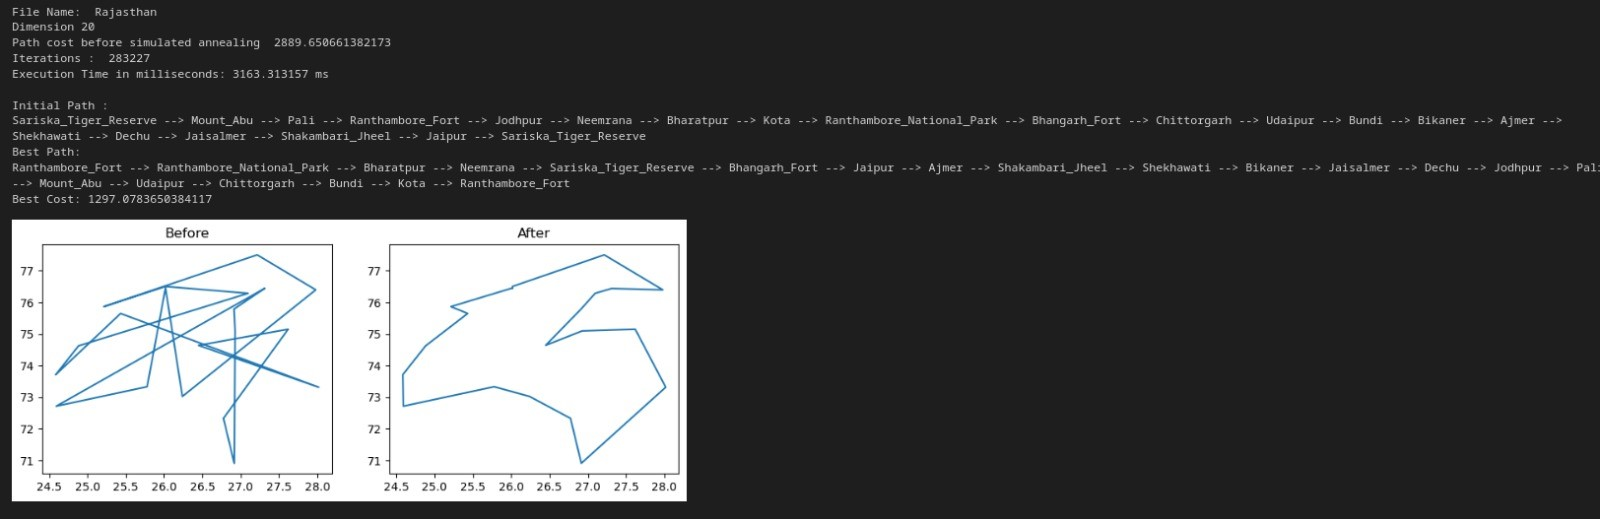
\includegraphics[scale=0.22]{images/3.1.jpg}\\
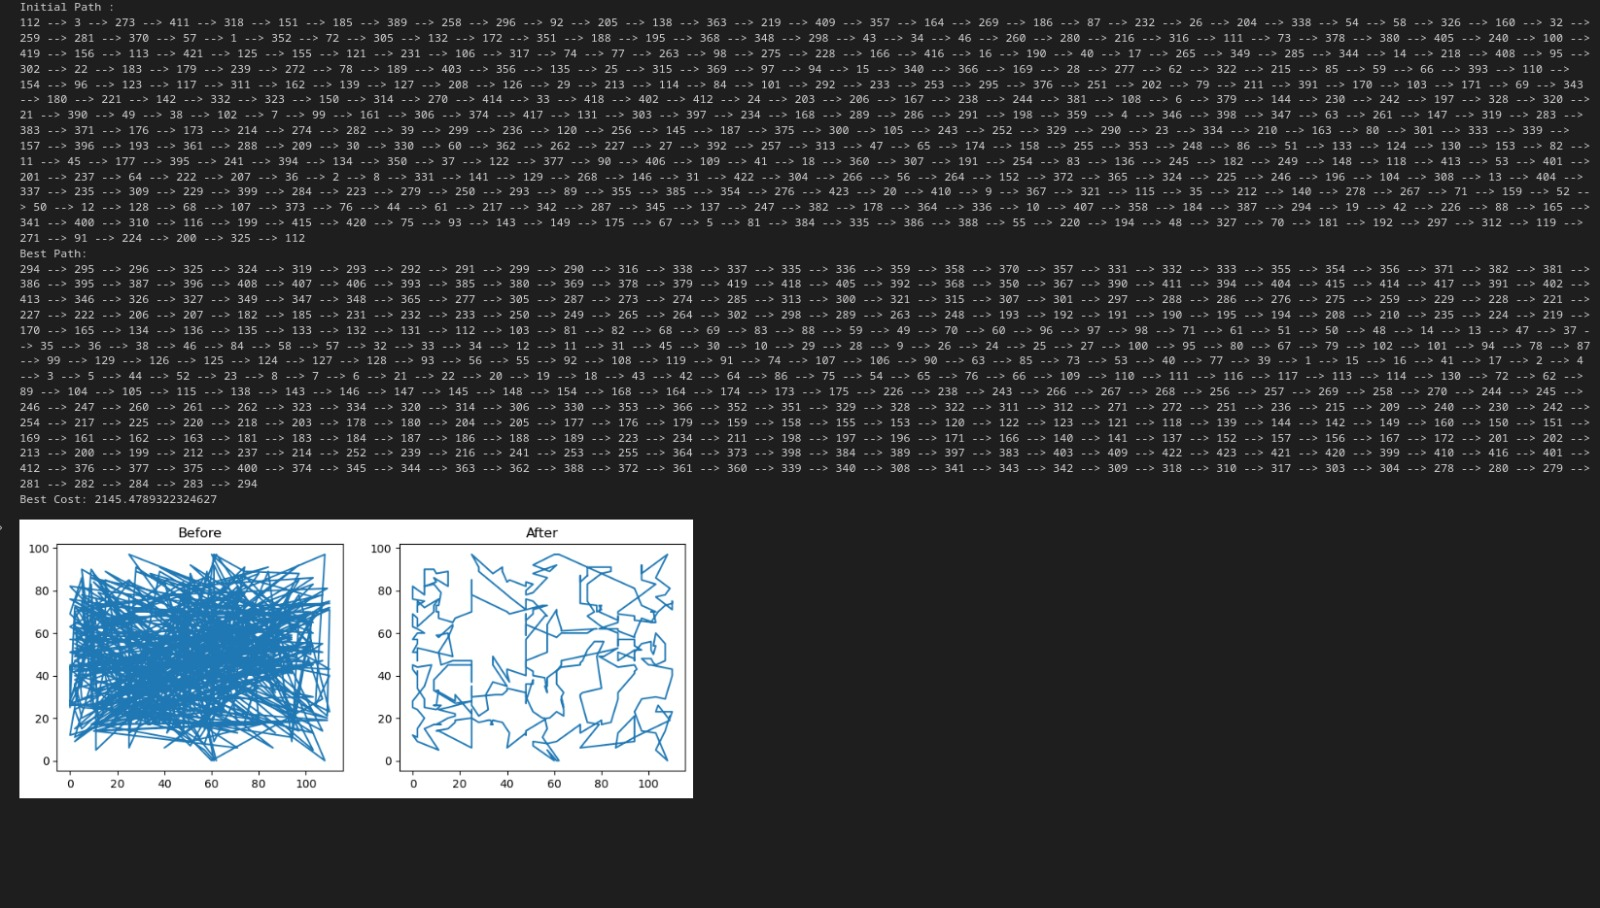
\includegraphics[scale=0.16]{images/3.2.jpg}\\
\section{Conclusion}
We successfully applied Simulated Annealing to the Traveling Salesman Problem and drastically decreased path cost. Simulated annealing, when configured appropriately and under specific circumstances, can guarantee finding the global optimum, whereas Hill Climbing/Descent can only make this promise if all local optima in the search space have equal scores and costs.

\begin{thebibliography}{9}
\bibitem{}
Deepak Khemani (2013) \emph{A First Course in Artificial Intelligence}, McGraw Hill Education (India) Private Limited, 1st ed.
\bibitem{}
 Stuart J. Russell and Peter
Norvig (2022) \emph{Artificial Intelligence - A Modern Approach}, Pearson Education Limited, 4th ed.
\bibitem{}
Tanmay Ambadkar (2021 Artificial Intelligence Course. \href{https://github.com/TanmayAmbadkar/CS302-AI/tree/master/Lab3}{https://github.com/TanmayAmbadkar/CS302-AI/tree/master/Lab3}(2023).
\end{thebibliography}

\end{document}


